\documentclass[12pt,a4paper]{article}

\usepackage[a4paper,margin=1in]{geometry}
\usepackage{graphicx}
\usepackage{booktabs}
\usepackage{amsmath,amssymb}
\usepackage{float}
\usepackage{hyperref}
\usepackage{xcolor}
\usepackage{enumitem}
\usepackage{fancyhdr}
\usepackage{longtable}

\hypersetup{colorlinks=true,linkcolor=blue,urlcolor=blue}

\pagestyle{fancy}
\fancyhf{}
\lhead{ICS1512}
\rhead{Machine Learning Algorithms Laboratory}
\cfoot{\thepage}

\begin{document}

\begin{tabular}{|p{4cm}|p{11cm}|}
\hline
Experiment No. & 3 \\ \hline
Experiment Title &
Loan Amount Prediction using Linear and Regularized Regression Models
\footnote{\textbf{GitHub Repository: }\url{https://github.com/JJBOY12345/MLAssign_SSN}}\\ \hline
Student Name & \\ \hline
Register Number & \\ \hline
Faculty & Dr. Poreddy Ajay Kumar Reddy \\ \hline
Submission Date & \\ \hline
\end{tabular}

\section{Objective}
TODO: State the objective of this experiment — to predict the loan sanction amount (in USD) using Linear Regression and regularized variants (Ridge, Lasso, ElasticNet), and to analyze the bias-variance trade-off through hyperparameter tuning.

\section{Problem Statement}
TODO: Describe the problem — given applicant details (income, education, employment, assets, CIBIL score, etc.), the task is to predict the loan sanction amount (a continuous variable). Discuss the input features, output (regression target), and objective (accurate loan amount prediction).

\section{Dataset Description}
\begin{longtable}{|p{5cm}|p{9cm}|}
\hline
Dataset Name & Loan Amount Prediction \\ \hline
Dataset Source & \texttt{predict\_loan\_amount/train.csv} and \texttt{test.csv} \\ \hline
Number of Samples (Train) & 30,000 (before cleaning) \\ \hline
Number of Samples (Test) & 20,000 (no target column) \\ \hline
Number of Features & 24 (before preprocessing), 45 (after preprocessing) \\ \hline
Target Variable & \texttt{Loan Sanction Amount (USD)} \\ \hline
Missing Values & Yes — multiple columns had missing values (handled via imputation) \\ \hline
Duplicate Records & None \\ \hline
Train-Test Split & 80\% Train (23,457), 20\% Test (5,865) from train.csv \\ \hline
\end{longtable}

TODO: Describe the dataset, its features, and the regression task.

\section{Exploratory Data Analysis}
For the Loan dataset, only basic information was examined (dataset info, missing values, duplicates, summary statistics). Visualizations were intentionally skipped.

\subsection{Dataset Overview}
TODO: Discuss the dataset shape, columns, data types, and initial observations.

\subsection{Missing Values and Duplicates}
TODO: Report findings — missing values detected in multiple columns (Income, Credit Score, Property Age, etc.), no duplicates found.

\subsection{Summary Statistics}
TODO: Present key statistics for numerical features.

\begin{longtable}{|l|r|r|r|r|}
\hline
\textbf{Feature} & \textbf{Mean} & \textbf{Std} & \textbf{Min} & \textbf{Max} \\ \hline
Age & 40.09 & 16.05 & 18 & 65 \\ \hline
Income (USD) & 2,630.57 & 11,262.72 & 377.70 & 1,777,460 \\ \hline
Loan Amount Request (USD) & 88,826.33 & 59,536.95 & 6,048.24 & 621,497.82 \\ \hline
Credit Score & 739.89 & 72.16 & 580 & 896.26 \\ \hline
Loan Sanction Amount (USD) & 47,649.34 & 48,221.15 & -999 & 481,907.32 \\ \hline
\end{longtable}

\section{Data Preprocessing}
Explain the preprocessing steps performed:

\subsection{Data Cleaning}
The \texttt{clean\_dataframe()} function handles:
\begin{itemize}
    \item Replacement of invalid values (\texttt{-999}, \texttt{"?"}, \texttt{"NA"}, etc.) with \texttt{NaN}.
    \item Dropping non-informative columns (\texttt{Customer ID}, \texttt{Name}).
    \item Converting columns to numeric where possible.
\end{itemize}

\subsection{Train-Test Split}
TODO: Explain that the data was split into 80\% training and 20\% testing before preprocessing to prevent data leakage.

\subsection{ColumnTransformer Pipeline}
A preprocessing pipeline was built using \texttt{ColumnTransformer}:
\begin{itemize}
    \item \textbf{Numeric Pipeline}: \texttt{SimpleImputer(strategy='median')} → \texttt{StandardScaler()}
    \item \textbf{Categorical Pipeline}: \texttt{SimpleImputer(strategy='most\_frequent')} → \texttt{OneHotEncoder(drop='first')}
\end{itemize}

\section{Machine Learning Algorithms}
Explain the working principle, mathematical formulation, advantages, and limitations of each algorithm:

\subsection{Linear Regression}
TODO: Explain Linear Regression — models the relationship between features and target as a linear combination, minimizes MSE.

\subsection{Ridge Regression (L2 Regularization)}
TODO: Explain Ridge — adds L2 penalty to the loss function to shrink coefficients, reduces variance.

\subsection{Lasso Regression (L1 Regularization)}
TODO: Explain Lasso — adds L1 penalty, performs feature selection by zeroing out less important coefficients.

\subsection{ElasticNet (L1 + L2 Regularization)}
TODO: Explain ElasticNet — combines L1 and L2 penalties, controlled by \texttt{alpha} and \texttt{l1\_ratio}.

\section{Experimental Setup}
\begin{tabular}{ll}
\toprule
Python Version & TODO: Specify \\
Scikit-Learn Version & TODO: Specify \\
IDE & TODO: Specify \\
Operating System & TODO: Specify \\
Hardware & TODO: Specify \\
\bottomrule
\end{tabular}

\section{Model 1: Linear Regression (Baseline)}
TODO: Explain training process.

\subsection{Results}
\begin{table}[H]
\centering
\begin{tabular}{lc}
\toprule
\textbf{Metric} & \textbf{Value} \\ \midrule
MAE & TODO \\
MSE & TODO \\
RMSE & TODO \\
R² Score & TODO \\
Training Time (s) & TODO \\
\bottomrule
\end{tabular}
\caption{Linear Regression Performance Metrics}
\end{table}

\subsection{Overfitting / Underfitting Analysis}
\begin{table}[H]
\centering
\begin{tabular}{lccc}
\toprule
\textbf{Model} & \textbf{Train R²} & \textbf{Test R²} & \textbf{Gap} \\ \midrule
Linear Regression & TODO & TODO & TODO \\
\bottomrule
\end{tabular}
\caption{Linear Regression — Train vs Test Performance}
\end{table}

\textbf{Inference:}
TODO: Discuss whether the model is overfitting or underfitting based on the R² gap.

\section{Model 2: Ridge Regression (Before Tuning)}
TODO: Explain training with default alpha=1.0.

\subsection{Results}
\begin{table}[H]
\centering
\begin{tabular}{lc}
\toprule
\textbf{Metric} & \textbf{Value} \\ \midrule
MAE & TODO \\
MSE & TODO \\
RMSE & TODO \\
R² Score & TODO \\
Training Time (s) & TODO \\
\bottomrule
\end{tabular}
\caption{Ridge Regression Performance Metrics (Default)}
\end{table}

\section{Model 3: Lasso Regression (Before Tuning)}
TODO: Explain training with default alpha=0.1.

\subsection{Results}
\begin{table}[H]
\centering
\begin{tabular}{lc}
\toprule
\textbf{Metric} & \textbf{Value} \\ \midrule
MAE & TODO \\
MSE & TODO \\
RMSE & TODO \\
R² Score & TODO \\
Training Time (s) & TODO \\
\bottomrule
\end{tabular}
\caption{Lasso Regression Performance Metrics (Default)}
\end{table}

\section{Model 4: ElasticNet (Before Tuning)}
TODO: Explain training with default alpha=0.1, l1\_ratio=0.5.

\subsection{Results}
\begin{table}[H]
\centering
\begin{tabular}{lc}
\toprule
\textbf{Metric} & \textbf{Value} \\ \midrule
MAE & TODO \\
MSE & TODO \\
RMSE & TODO \\
R² Score & TODO \\
Training Time (s) & TODO \\
\bottomrule
\end{tabular}
\caption{ElasticNet Performance Metrics (Default)}
\end{table}

\section{Hyperparameter Tuning}
\subsection{Ridge — GridSearchCV}
\begin{longtable}{|l|l|}
\hline
\textbf{Parameter} & \textbf{Values Searched} \\ \hline
alpha & 0.01, 0.1, 1, 10, 100 \\ \hline
\end{longtable}

TODO: Report best alpha and best CV R² score.

\subsection{Lasso — GridSearchCV}
\begin{longtable}{|l|l|}
\hline
\textbf{Parameter} & \textbf{Values Searched} \\ \hline
alpha & 0.001, 0.01, 0.1, 1, 10 \\ \hline
\end{longtable}

TODO: Report best alpha and best CV R² score.

\subsection{ElasticNet — GridSearchCV}
\begin{longtable}{|l|l|}
\hline
\textbf{Parameter} & \textbf{Values Searched} \\ \hline
alpha & 0.01, 0.1, 1, 10 \\ \hline
l1\_ratio & 0.2, 0.5, 0.8 \\ \hline
\end{longtable}

TODO: Report best alpha, best l1\_ratio, and best CV R² score.

\subsection{Hyperparameter Tuning Summary}
\begin{table}[H]
\centering
\begin{tabular}{lccc}
\toprule
\textbf{Model} & \textbf{Best Params} & \textbf{Best CV R²} & \textbf{Grid Time (s)} \\ \midrule
Ridge & TODO & TODO & TODO \\
Lasso & TODO & TODO & TODO \\
ElasticNet & TODO & TODO & TODO \\
\bottomrule
\end{tabular}
\caption{GridSearchCV Results Summary}
\end{table}

\section{Tuned Model Results}
\subsection{Performance Comparison: Before vs After Tuning}
\begin{table}[H]
\centering
\begin{tabular}{lcccc}
\toprule
\textbf{Model} & \textbf{MAE} & \textbf{RMSE} & \textbf{R²} & \textbf{Train Time (s)} \\ \midrule
Ridge (Default) & TODO & TODO & TODO & TODO \\
Ridge (Tuned) & TODO & TODO & TODO & TODO \\
Lasso (Default) & TODO & TODO & TODO & TODO \\
Lasso (Tuned) & TODO & TODO & TODO & TODO \\
ElasticNet (Default) & TODO & TODO & TODO & TODO \\
ElasticNet (Tuned) & TODO & TODO & TODO & TODO \\
\bottomrule
\end{tabular}
\caption{Performance Comparison — Default vs Tuned Models}
\end{table}

\section{Result Visualization}

\subsection{Predicted vs Actual Values}
\begin{figure}[H]
\centering
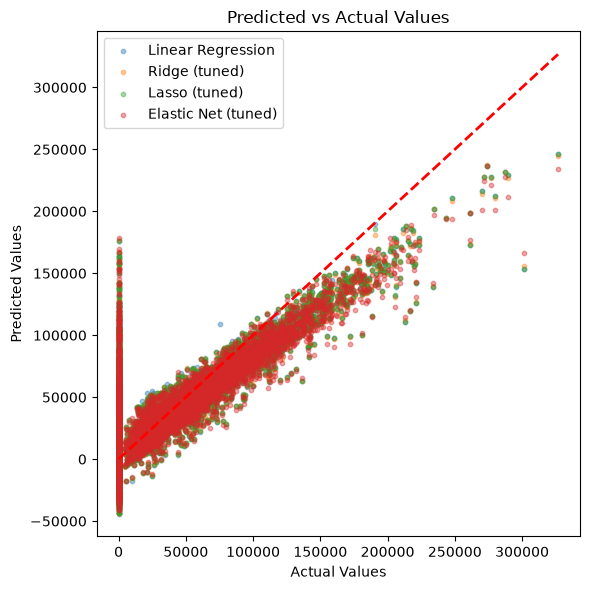
\includegraphics[width=0.7\linewidth]{images/predicted_vs_actual.png}
\caption{Predicted vs Actual Values for All Models}
\end{figure}

\textbf{Inference:}
TODO: Discuss how closely the predicted values align with the ideal diagonal line. Which model shows the best fit?

\subsection{Residual Plot}
\begin{figure}[H]
\centering
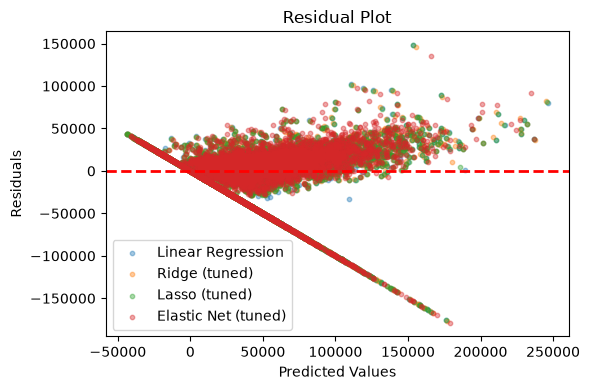
\includegraphics[width=0.7\linewidth]{images/residual_plot.png}
\caption{Residual Plot — Predicted vs Residuals}
\end{figure}

\textbf{Inference:}
TODO: Discuss the pattern of residuals — are they randomly distributed around zero? Check for heteroscedasticity.

\subsection{Coefficient Comparison}
\begin{figure}[H]
\centering
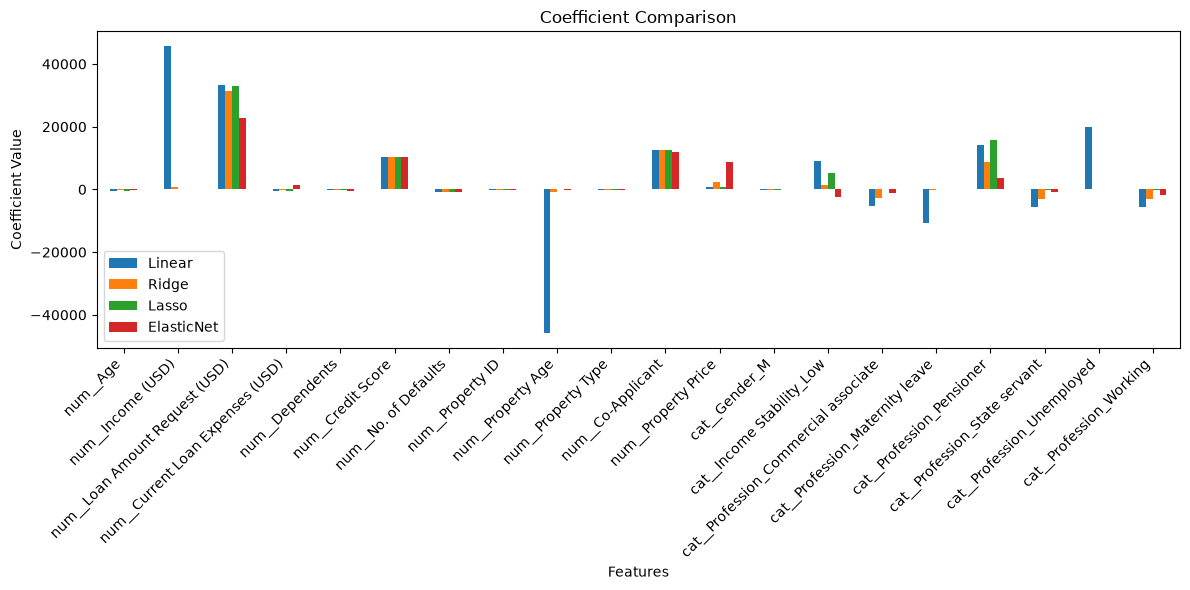
\includegraphics[width=0.7\linewidth]{images/coefficient_comparison.png}
\caption{Coefficient Comparison Across Models (Top 20 Features)}
\end{figure}

\textbf{Inference:}
TODO: Compare how coefficients vary across models — note how Lasso zeroes out some features, while Ridge shrinks them.

\subsection{Training vs Validation Error (5-Fold CV)}
\begin{figure}[H]
\centering
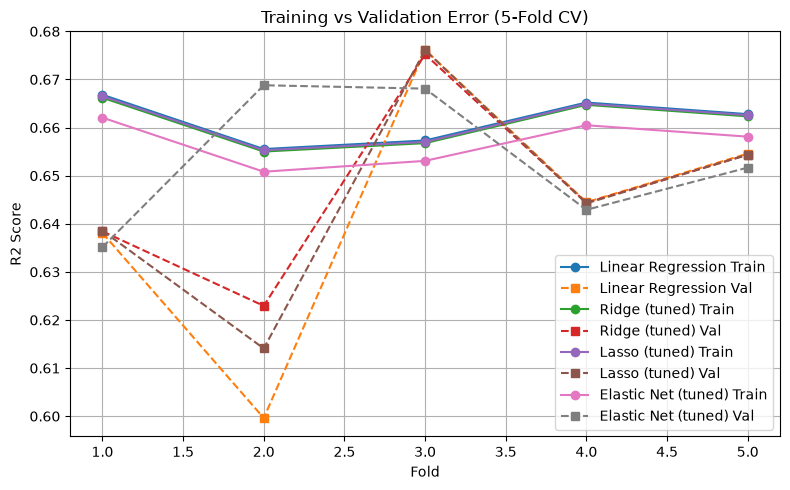
\includegraphics[width=0.7\linewidth]{images/train_vs_validation_error.png}
\caption{Training vs Validation R² Scores Across 5 Folds}
\end{figure}

\textbf{Inference:}
TODO: Discuss the gap between training and validation scores — identify any overfitting.

\section{Cross-Validation Performance}
\begin{table}[H]
\centering
\begin{tabular}{lcccc}
\toprule
\textbf{Model} & \textbf{MAE} & \textbf{MSE} & \textbf{RMSE} & \textbf{R²} \\ \midrule
Linear Regression & TODO & TODO & TODO & TODO \\
Ridge (Tuned) & TODO & TODO & TODO & TODO \\
Lasso (Tuned) & TODO & TODO & TODO & TODO \\
ElasticNet (Tuned) & TODO & TODO & TODO & TODO \\
\bottomrule
\end{tabular}
\caption{5-Fold Cross-Validation Performance}
\end{table}

\section{Coefficient Comparison Table}
TODO: Present a table showing the coefficients of each model for the top features.

\begin{longtable}{lcccc}
\toprule
\textbf{Feature} & \textbf{Linear} & \textbf{Ridge} & \textbf{Lasso} & \textbf{ElasticNet} \\ \midrule
TODO & TODO & TODO & TODO & TODO \\
TODO & TODO & TODO & TODO & TODO \\
TODO & TODO & TODO & TODO & TODO \\
\bottomrule
\end{longtable}

\textbf{Inference:}
TODO: Discuss how regularization affects coefficient magnitudes — Lasso drives some to zero.

\section{Overfitting and Underfitting Analysis}
\begin{table}[H]
\centering
\begin{tabular}{lccc}
\toprule
\textbf{Model} & \textbf{Train R²} & \textbf{Test R²} & \textbf{Gap} \\ \midrule
Linear Regression & TODO & TODO & TODO \\
Ridge (Tuned) & TODO & TODO & TODO \\
Lasso (Tuned) & TODO & TODO & TODO \\
ElasticNet (Tuned) & TODO & TODO & TODO \\
\bottomrule
\end{tabular}
\caption{Overfitting / Underfitting Analysis}
\end{table}

\textbf{Inference:}
TODO: Discuss which models show signs of overfitting (large gap) and which are well-balanced.

\section{Bias-Variance Analysis}
TODO: Discuss the bias-variance trade-off for each model:

\begin{itemize}
    \item \textbf{Linear Regression}: High bias (linear assumption), low variance.
    \item \textbf{Ridge Regression}: Reduces variance by shrinking coefficients, slightly increases bias.
    \item \textbf{Lasso Regression}: Feature sparsity — zeroes out less important features, performs feature selection.
    \item \textbf{ElasticNet}: Combines L1 and L2 regularization, balances bias-variance trade-off.
\end{itemize}

\section{Discussion}
TODO: Discuss observations, strengths, and limitations:
\begin{itemize}
    \item Overall best performing model and why.
    \item Effect of regularization on model performance.
    \item Impact of hyperparameter tuning (alpha, l1\_ratio).
    \item Feature selection capability of Lasso vs Ridge.
    \item Bias-variance trade-off observed across models.
\end{itemize}

\section{Conclusion}
TODO: Summarize the experiment — Linear Regression and its regularized variants (Ridge, Lasso, ElasticNet) were applied to predict loan sanction amounts. Hyperparameter tuning was performed using GridSearchCV. Model performance was evaluated using MAE, MSE, RMSE, R², and cross-validation. The bias-variance trade-off and overfitting characteristics were analyzed.

\section{References}
\begin{enumerate}
    \item TODO: Reference scikit-learn documentation for Linear, Ridge, Lasso, ElasticNet regression.
    \item TODO: Reference pandas, Matplotlib, and Seaborn documentation.
    \item TODO: Reference documentation on GridSearchCV and ColumnTransformer.
\end{enumerate}

\end{document}